\documentclass{ximera}

\title{Practice for Chaos}

%\auor{Matthew Charnley and Jason Nowell}
\usepackage[margin=1.5cm]{geometry}
\usepackage{indentfirst}
\usepackage{sagetex}
\usepackage{lipsum}
\usepackage{amsmath}
\usepackage{mathrsfs}


%%% Random packages added without verifying what they are really doing - just to get initial compile to work.
\usepackage{tcolorbox}
\usepackage{hypcap}
\usepackage{booktabs}%% To get \toprule,\midrule,\bottomrule etc.
\usepackage{nicefrac}
\usepackage{caption}
\usepackage{units}

% This is my modified wrapfig that doesn't use intextsep
\usepackage{mywrapfig}
\usepackage{import}



%%% End to random added packages.


\graphicspath{
    {./figures/}
    {./../figures/}
    {./../../figures/}
}
\renewcommand{\log}{\ln}%%%%
\DeclareMathOperator{\arcsec}{arcsec}
%% New commands


%%%%%%%%%%%%%%%%%%%%
% New Conditionals %
%%%%%%%%%%%%%%%%%%%%


% referencing
\makeatletter
    \DeclareRobustCommand{\myvref}[2]{%
      \leavevmode%
      \begingroup
        \let\T@pageref\@pagerefstar
        \hyperref[{#2}]{%
	  #1~\ref*{#2}%
        }%
        \vpageref[\unskip]{#2}%
      \endgroup
    }%

    \DeclareRobustCommand{\myref}[2]{%
      \leavevmode%
      \begingroup
        \let\T@pageref\@pagerefstar
        \hyperref[{#2}]{%
	  #1~\ref*{#2}%
        }%
      \endgroup
    }%
\makeatother

\newcommand{\figurevref}[1]{\myvref{Figure}{#1}}
\newcommand{\figureref}[1]{\myref{Figure}{#1}}
\newcommand{\tablevref}[1]{\myvref{Table}{#1}}
\newcommand{\tableref}[1]{\myref{Table}{#1}}
\newcommand{\chapterref}[1]{\myref{chapter}{#1}}
\newcommand{\Chapterref}[1]{\myref{Chapter}{#1}}
\newcommand{\appendixref}[1]{\myref{appendix}{#1}}
\newcommand{\Appendixref}[1]{\myref{Appendix}{#1}}
\newcommand{\sectionref}[1]{\myref{\S}{#1}}
\newcommand{\subsectionref}[1]{\myref{subsection}{#1}}
\newcommand{\subsectionvref}[1]{\myvref{subsection}{#1}}
\newcommand{\exercisevref}[1]{\myvref{Exercise}{#1}}
\newcommand{\exerciseref}[1]{\myref{Exercise}{#1}}
\newcommand{\examplevref}[1]{\myvref{Example}{#1}}
\newcommand{\exampleref}[1]{\myref{Example}{#1}}
\newcommand{\thmvref}[1]{\myvref{Theorem}{#1}}
\newcommand{\thmref}[1]{\myref{Theorem}{#1}}


\renewcommand{\exampleref}[1]{ {\color{red} \bfseries Normally a reference to a previous example goes here.}}
\renewcommand{\figurevref}[1]{ {\color{red} \bfseries Normally a reference to a previous figure goes here.}}
\renewcommand{\tablevref}[1]{ {\color{red} \bfseries Normally a reference to a previous table goes here.}}
\renewcommand{\Appendixref}[1]{ {\color{red} \bfseries Normally a reference to an Appendix goes here.}}
\renewcommand{\exercisevref}[1]{ {\color{red} \bfseries Normally a reference to a previous exercise goes here.}}



\newcommand{\R}{\mathbb{R}}

%% Example Solution Env.
\def\beginSolclaim{\par\addvspace{\medskipamount}\noindent\hbox{\bf Solution:}\hspace{0.5em}\ignorespaces}
\def\endSolclaim{\par\addvspace{-1em}\hfill\rule{1em}{0.4pt}\hspace{-0.4pt}\rule{0.4pt}{1em}\par\addvspace{\medskipamount}}
\newenvironment{exampleSol}[1][]{\beginSolclaim}{\endSolclaim}

%% General figure formating from original book.
\newcommand{\mybeginframe}{%
\begin{tcolorbox}[colback=white,colframe=lightgray,left=5pt,right=5pt]%
}
\newcommand{\myendframe}{%
\end{tcolorbox}%
}

%%% Eventually return and fix this to make matlab code work correctly.
%% Define the matlab environment as another code environment
%\newenvironment{matlab}
%{% Begin Environment Code
%{ \centering \bfseries Matlab Code }
%\begin{code}
%}% End of Begin Environment Code
%{% Start of End Environment Code
%\end{code}
%}% End of End Environment Code


% this one should have a caption, first argument is the size
\newenvironment{mywrapfig}[2][]{
 \wrapfigure[#1]{r}{#2}
 \mybeginframe
 \centering
}{%
 \myendframe
 \endwrapfigure
}

% this one has no caption, first argument is size,
% the second argument is a larger size used for HTML (ignored by latex)
\newenvironment{mywrapfigsimp}[3][]{%
 \wrapfigure[#1]{r}{#2}%
 \centering%
}{%
 \endwrapfigure%
}
\newenvironment{myfig}
    {%
    \begin{figure}[h!t]
        \mybeginframe%
        \centering%
    }
    {%
        \myendframe
    \end{figure}%
    }


% graphics include
\newcommand{\diffyincludegraphics}[3]{\includegraphics[#1]{#3}}
\newcommand{\myincludegraphics}[3]{\includegraphics[#1]{#3}}
\newcommand{\inputpdft}[1]{\subimport*{../figures/}{#1.pdf_t}}


%% Not sure what these even do? They don't seem to actually work... fun!
%\newcommand{\mybxbg}[1]{\tcboxmath[colback=white,colframe=black,boxrule=0.5pt,top=1.5pt,bottom=1.5pt]{#1}}
%\newcommand{\mybxsm}[1]{\tcboxmath[colback=white,colframe=black,boxrule=0.5pt,left=0pt,right=0pt,top=0pt,bottom=0pt]{#1}}
\newcommand{\mybxsm}[1]{#1}
\newcommand{\mybxbg}[1]{#1}

%%% Something about tasks for practice/hw?
\usepackage{tasks}
\usepackage{footnote}
\makesavenoteenv{tasks}


%% For pdf only?
\newcommand{\diffypdfversion}[1]{#1}


%% Kill ``cite'' and go back later to fix it.
\renewcommand{\cite}[1]{}


%% Currently we can't really use index or its derivatives. So we are gonna kill them off.
\renewcommand{\index}[1]{}
\newcommand{\myindex}[1]{#1}







\begin{document}
\begin{abstract}
Why?
\end{abstract}
\maketitle


\begin{exercise}%[*]
    Find critical points of the Lorenz system and the associated linearizations.
\end{exercise}
%\exsol{%
%Critical points: $(0,0,0)$, $(3\sqrt{8},3 \sqrt{8}, 27)$,
%$(-3 \sqrt{8},-3 \sqrt{8}, 27)$.
%Linearization at $(0,0,0)$ using $u=x$, $v=y$, $w=z$ is
%$u' = -10u+10v$, $v'=28u-v$, $w'=-(\frac{8}{3})w$.
%Linearization at $(3 \sqrt{8},3\sqrt{8},27)$ using $u=x-3\sqrt{8}$,
%$v=y-3\sqrt{8}$, $w=z-27$ is
%$u' = -10u+10v$, $v'=u-v-3\sqrt{8}w$, $w'=3\sqrt{8}u+3\sqrt{8}v-(\frac{8}{3})w$.
%Linearization at $(-3 \sqrt{8},-3\sqrt{8},27)$ using $u=x+3\sqrt{8}$,
%$v=y+3\sqrt{8}$, $w=z-27$ is
%$u' = -10u+10v$, $v'=u-v+3\sqrt{8}w$, $w'=-3\sqrt{8}u-3\sqrt{8}v-(\frac{8}{3})w$.
%}

\begin{exercise}
    For the non-chaotic equation $x''+2p x' + \omega_0^2 x = \frac{F_0}{m} \cos (\omega t)$, suppose we strobe with frequency $\omega$ as we mentioned above.  Use the known steady periodic solution to find precisely the point which is the attractor for the Poincar\'e section.\\
    $(A, \omega B)$ for $A \answer{\cos(\omega t)} + B \answer{\sin(\omega t)}$, or $\answer{\frac{F_0/m}{(\omega_0^2 - \omega^2)^2 + (2p\omega)^2}(\omega_0^2 - \omega^2, 2p\omega^2)}$
\end{exercise}
%\comboSol
%{%
%$(A, \omega B)$ for $A \cos(\omega t) + B\sin(\omega t)$, or $\frac{F_0/m}{(\omega_0^2 - \omega^2)^2 + (2p\omega)^2}(\omega_0^2 - \omega^2, 2p\omega^2)$
%}

\begin{exercise}%[project]
    Construct the double pendulum described in the text with a string and two nuts (or heavy beads).  Play around with the position of the middle nut, and perhaps use different weight nuts.  Describe what you find.
\end{exercise}


\begin{exercise}%[project]
    A simple fractal attractor can be drawn via the following chaos game.  Draw the three vertices of a triangle and label them, say $p_1$, $p_2$ and $p_3$.  Draw some random point $p$ (it does not have to be one of the three points above). Roll a die to pick of the $p_1$, $p_2$, or $p_3$ randomly (for example 1 and 4 mean $p_1$, 2 and 5 mean $p_2$, and 3 and 6 mean $p_3$).  Suppose we picked $p_2$, then let $p_{\text{new}}$ be the point exactly halfway between $p$ and $p_2$.  Draw this point and let $p$ now refer to this new point $p_{\text{new}}$.  Rinse, repeat.  Try to be precise and draw as many iterations as possible.  Your points will be attracted to the so-called \emph{\myindex{Sierpinski triangle}}.  A computer was used to run the game for 10,000 iterations to obtain the picture in the figure below.
\end{exercise}

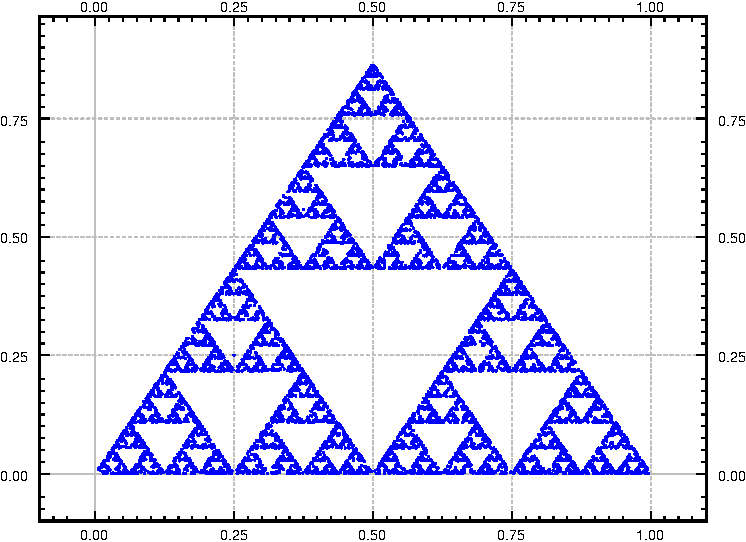
\includegraphics{nlin-sierpinski}
%\begin{myfig}
%    \diffyincludegraphics{width=3in}{width=4.5in}{nlin-sierpinski}
%    \caption{10,000 iterations of the chaos game producing the Sierpinski triangle. \label{nlin:sierpinski}}
%\end{myfig}


\begin{exercise}%[computer project]
    Use a computer software (such as Matlab, Octave, or perhaps even a spreadsheet), plot the solution of the given forced Duffing equation with Euler's method.  Plotting the solution for $t$ from 0 to 100 with several different (small) step sizes. Discuss.
\end{exercise}
%\comboSol
%{%
%You should get very different behavior for similar (small) step sizes becasue the equation is chaotic. 
%}

\end{document}